\documentclass[a4paper,11pt]{exam}
	\usepackage{graphicx}
	\usepackage[utf8]{inputenc}
	\usepackage[T1]{fontenc}
	\usepackage{listings}
	\usepackage{color}
	\usepackage{amsmath}
	\usepackage{enumerate}
	\usepackage{caption}
	\usepackage{verbatim}
	\usepackage{subcaption}
	\usepackage{tikz}
	\usepackage{graphics}
	\usepackage{txfonts}
	\usepackage{listings}
	\definecolor{dkgreen}{rgb}{0,0.5,0}
	\definecolor{gray}{rgb}{0.5,0.5,0.5}
	\definecolor{mauve}{rgb}{0.58,0,0.82}

	\lstset{frame=tb,
	  language=Python,
	  aboveskip=3mm,
	  belowskip=3mm,
	  showstringspaces=false,
	  columns=flexible,
	  basicstyle={\small\ttfamily},
	  numbers=none,
	  numberstyle=\tiny\color{gray},
	  keywordstyle=\color{blue},
	  commentstyle=\color{dkgreen},
	  stringstyle=\color{mauve},
	  breaklines=true,
	  breakatwhitespace=true
	  tabsize=3
	  }
	

\begin{document}
\begingroup 
	  \bf \Large Eletromagnetismo\\
	  \indent \normalsize André Del Bianco Giuffrida
	\endgroup
	\\ \quad
	\\
	\large{
	\emph{Lista 1 \\ Ex 1}
	\\
	\\
	Duas cargas pontuais, $+q$ e $-q$, estão situadas ao longo do eixo $x$ em $x=-\frac{d}{2}$ e $x = +\frac{d}{2}$, respectivamente.
	\\
	(a) Escreva uma expressão para a densidade de carga $\rho(\vec{r})$ em todo o espaço.
	\\
	(b) Calcule o potencial elétrico ao longo do eixo $z$.
	\\
	(c) A partir do resultado do item (b), calcule o vetor campo elétrico ao longo do eixo $z$.
	\\
	\\
	\normalsize
	
	\begin{center}
		\begin{tikzpicture}
			\draw (-6,0) -- (6,0);
			\draw[arrows=<->] (-3,-2)--(3,-2);
			\draw (-3,0.1)--(-3,-2.3);
			\draw (3,0.1)--(3,-2.3);
			\node at (0,-0.4) {0};
			\draw[fill=black] (3,0) circle (.1);
			\node at (3,0.5) {$-q$};
			\draw[fill=black] (-3,0) circle (.1);
			\node at (-3,0.5) {$+q$};
			\node at (0,0) {|};
			\node[fill=white,font=\footnotesize,inner sep=3pt] at (0,-2) {$d$};
		\end{tikzpicture}
	\end{center}
	
	Usando a função delta de dirac podemos construir a densidade de carga espacial
	\[ \rho(\vec{r}) = +q \Big( \delta(\vec{r} + \frac{d}{2} \hat{x} ) - \delta(\vec{r} - \frac{d}{2} \hat{x} ) \Big)  \]
	\indent Para confirmar basta integrar $\rho(\vec{r})$ em todo o espaço 
	\[Q = \int_{V} \rho(\vec{r'}) dv'= \int_{V} q\delta(\vec{r} + \frac{d}{2} \hat{x} )dv' - \int_{V} q\delta(\vec{r} - \frac{d}{2} \hat{x} )dv' = q - q = 0\]
	como já era esperado a carga total $Q$ em todo espaço é nula 
	\\
	\\
	\indent Para calcular o potencial elétrico ao longo do eixo z vamos utilizar o principio de superposição e o potencial para uma única carga pontual.
	\[V_u(\vec{r}) = \frac{1}{4 \pi \epsilon_0} \frac{q}{|(\vec{r} - \vec{r_i})|} \]
	\indent Onde $\vec{r_i}$ é a coordenada da carga, usando o princípio de superposição podemos escrever:
	\[ V(\vec{r}) = \frac{1}{4 \pi \epsilon_0} \Bigg( \frac{q}{|\vec{r} - \frac{d}{2}\hat{x}|}  + \frac{-q}{|\vec{r} + \frac{d}{2}\hat{x}|} \Bigg)\]
	\indent Ao longo do eixo z temos que $\vec{r} = 0\hat{x} + 0\hat{y} + z\hat{z} $
	\[ V(z) = \frac{1}{4 \pi \epsilon_0} \Bigg( \frac{q}{\sqrt{z^2 +\frac{d^2}{4}}}  + \frac{-q}{\sqrt{z^2 + \frac{d^2}{4}}} \Bigg) \quad = \quad  \frac{1}{4 \pi \epsilon_0} \Bigg( \frac{q - q}{\sqrt{z^2 +\frac{d^2}{4}}} \Bigg) \quad = \quad 0\]
	\indent Ou seja o Potencial elétrico ao longo do eixo $z$ é nulo
	Usando agora a definição de potencial para calcular $\vec{E}$
	\[\vec{E}(\vec{r}) = -\nabla V(r) \]
	Aplicando o gradiente em $V(r)$
	\[\vec{E} = \frac{-1}{4 \pi \epsilon_0}  \nabla \Bigg( \frac{q}{|\vec{r} - \frac{d}{2}\hat{x}|}  + \frac{-q}{|\vec{r} + \frac{d}{2}\hat{x}|} \Bigg)\]
	\[\vec{E} = \frac{-1}{4 \pi \epsilon_0}\nabla \Bigg( \frac{q}{\sqrt{(x-\frac{d}{2})^2 + y^2 + z^2 }}  + \frac{-q}{\sqrt{(x+\frac{d}{2})^2 + y^2 + z^2 }} \Bigg)\]
	\[\vec{E} = \frac{-1}{4 \pi \epsilon_0}\nabla \Bigg( \frac{q}{\sqrt{x^2 +\frac{d^2}{4} - xd + y^2 + z^2 }}  + \frac{-q}{\sqrt{x^2 +\frac{d^2}{4} + xd + y^2 + z^2 }} \Bigg)\]
	
	Usando a seguinte identidade para a derivada:
	\[\frac{\partial }{\partial x} \frac{1}{\sqrt{x^2 + xa + c}} = -\frac{(a+2 x)}{(2(c + x (a+x))^{\frac{3}{2}})} \]
	\indent Podemos escrever separadamente
	
	\[E_x=\frac{-q(a+2x)}{2(x(a+x)+c)^{\frac{3}{2}}}+\frac{q(a-2x)}{2(x(x-a)+c)^{\frac{3}{2}}}\hat{x}\]
	
	\begin{figure}[h]
		\centering
		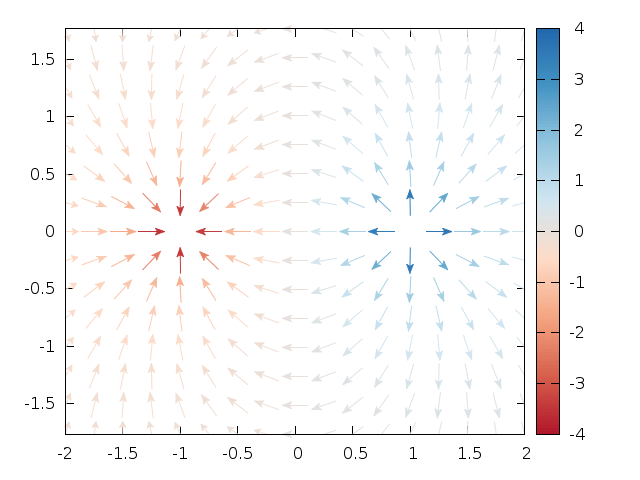
\includegraphics[scale=0.7]{Field.png}
		\caption{ }
	\end{figure} 
	
\end{document}
